\section{Experience}
\label{sect:results}



The blockchain has slowly attracted more traffic and we can now see over 1000
transactions an hour on busy days (Fig.\ \ref{txs-nrs}).
\begin{figure}[h]
   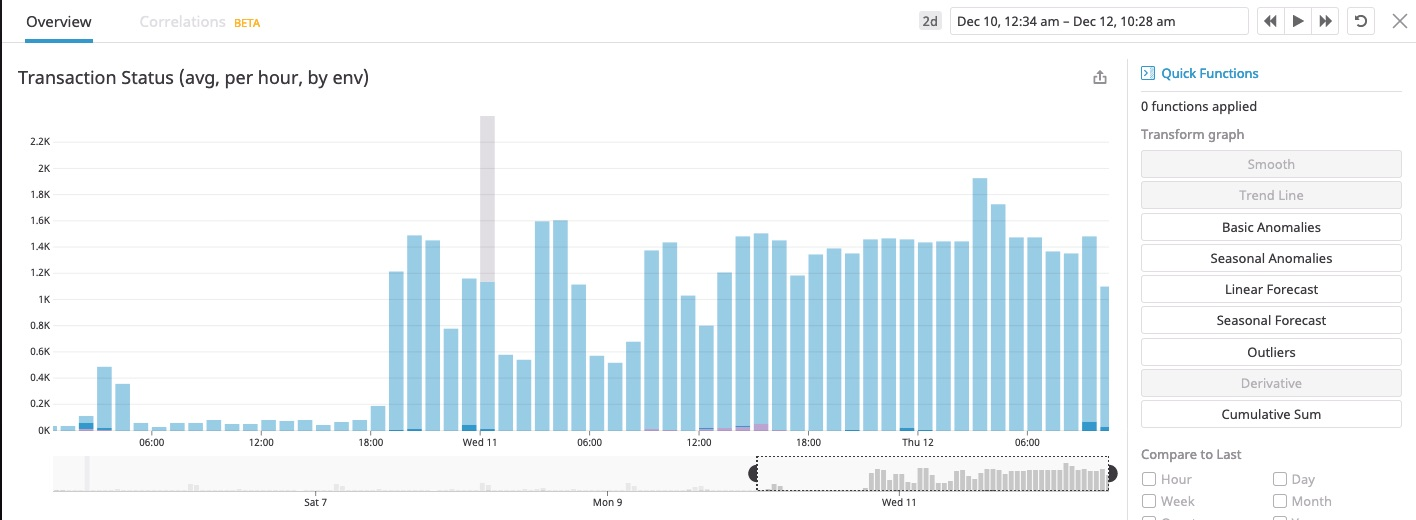
\includegraphics[scale=0.23]{TransactionsDec2019.jpg}
   \caption{Transaction status}
   \label{txs-nrs}
\end{figure}
This is much below the theoretical maximum of 100 on-chain transaction per
second.

The confirmation time of transactions is the time between posting the
transaction and seeing it in a micro-block on chain. We measure this over a
longer time by posting a transaction each 3 seconds carrying the post time as
timestamp in the payload. The micro-block in which this transaction appears
also has a timestamp (set by the clock of the miner). The difference is
observable for everyone, since these are transactions on chain. The mean of
confirmation times is around the expected 3 seconds.


